\section{Numerical Examples}
In the following examples, units are omitted for brevity.
\subsection{SDOF System With Single Exponential}
We start with the validation of \algoref{algo:single_model}. To this end, consider the free vibration of a SDOF system with one exponential kernel such that the EOM can be expressed as
\begin{gather}
m\ddot{u}\left(t\right)+\int_0^tc\mu\exp\left(-\mu\left(t-\tau\right)\right)\dot{u}\left(\tau\right)\md{\tau}+ku\left(t\right)=0.
\end{gather}
The parameters are set to $m=1$, $c=2$, $\mu=1$, $k=100$.
The initial conditions are $u\left(0\right)=1$, $\dot{u}\left(0\right)=1$ and $\ddot{u}\left(0\right)=1$.
The closed form solution can be found in \secref{sec:analytical_sdof}.
The Newmark (constant acceleration) method is used for time integration.
The displacement history and the corresponding error convergence are shown in \figref{fig:sdof}.

The maximum of the difference between numerical and analytical solutions is taken as the absolute error $\epsilon$. It is evident that \eqsref{eq:discretised_c} retains the second-order accuracy of the Newmark method.
\begin{figure}[H]
\centering
\includegraphics{PY/single_exp}
\caption{displacement history and error analysis of SDOF oscillator with one exponential kernel}\label{fig:sdof}
\end{figure}
\subsection{Three DOF System With Two Exponentials}
A three-degree-of-freedom system shown in \figref{fig:three_dof} is adopted to demonstrate the applicability of the proposed algorithm in MDOF systems. This example is also adopted by some of aforementioned work \cite[see, e.g.,][]{Adhikari2004,Cortes2009,Shen2019,Liu2023}.
\begin{figure}[H]
\centering
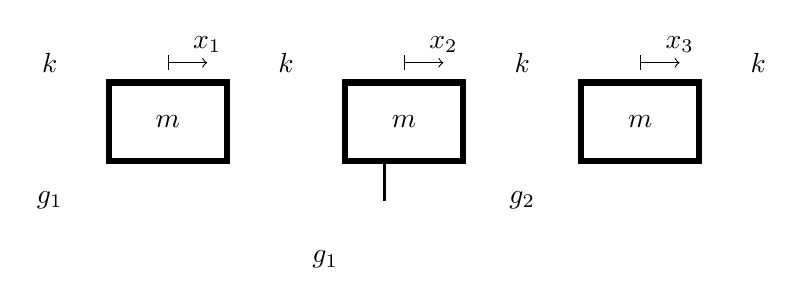
\begin{tikzpicture}
\draw[line width=.8mm](2,0)rectangle++(1.5,1);
\draw[line width=.8mm](5,0)rectangle++(1.5,1);
\draw[line width=.8mm](8,0)rectangle++(1.5,1);
\setstructmech{linewidth=.4mm}
\Spring{.5,.75}{2,.75}{1.5}
\Spring{3.5,.75}{5,.75}{1.5}
\Spring{6.5,.75}{8,.75}{1.5}
\Spring{9.5,.75}{11,.75}{1.5}
\Dashpot{6.5,.25}{8,.25}{1.5}
\Dashpot{.5,.25}{2,.25}{1.5}
\Dashpot{4,-.5}{5.5,-.5}{1.5}
\FixedSupport[-90]{.5,.5}{2}
\FixedSupport[90]{11,.5}{2}
\FixedSupport[-90]{4,-.5}
\draw[line width=.4mm](5.5,-.5)--++(0,.5);
\draw[|->](2.75,1.25)--++(.5,0)node[above]{$x_1$};
\draw[|->](5.75,1.25)--++(.5,0)node[above]{$x_2$};
\draw[|->](8.75,1.25)--++(.5,0)node[above]{$x_3$};
\node at(2.75,.5){$m$};
\node at(5.75,.5){$m$};
\node at(8.75,.5){$m$};
\node at(1.25,1.25){$k$};
\node at(4.25,1.25){$k$};
\node at(7.25,1.25){$k$};
\node at(10.25,1.25){$k$};
\node at(1.25,-.5){$g_1$};
\node at(4.75,-1.25){$g_1$};
\node at(7.25,-.5){$g_2$};
\end{tikzpicture}
\caption{three DOF system with two exponential kernels}\label{fig:three_dof}
\end{figure}
The parameters are set to $m=3$, $k=2$ and
\begin{gather}
g_1=\num{0.6}\exp\left(-t\right),\qquad
g_2=\exp\left(-\num{5}t\right).
\end{gather}
The initial conditions are $x_1\left(0\right)=1$, $x_2\left(0\right)=x_3\left(0\right)=0$, and $\dot{x}_1\left(0\right)=\dot{x}_2\left(0\right)=\dot{x}_3\left(0\right)=0$. One can compute the initial acceleration using the analytical solution such that $\ddot{x}_1\left(0\right)=-4/3$, $\ddot{x}_2\left(0\right)=2/3$ and $\ddot{x}_3\left(0\right)=0$.
The analytical solution can be obtained via modal analysis/expansion, the relevant derivations can be seen elsewhere \citep[see][\S~4.6.2]{Adhikari2014}.
The Newmark (constant acceleration) method is used for time integration.

The displacement histories of three DoFs are depicted in \figref{fig:three}.
\begin{figure}[H]
\centering
\includegraphics{PY/three_dof}
\caption{displacement history and error analysis of three DOF system with two exponential kernels}\label{fig:three}
\end{figure}


Compared to the numerical solutions (with $\Delta{}t=\SI{0.05}{\second}$) obtained by \citet{Cortes2009}, the present algorithm yields more accurate results. Even for a large time step $\Delta{}t=\SI{0.1}{\second}$, unlike other methods \citep{Liu2023}, there is no severe deviation observed.

The convergence of absolute error again shows a quadratic order, implying the simple \eqsref{eq:eqv_sys} is effective.


\begin{figure}
\centering
\begin{subfigure}[b]{0.49\textwidth}
\centering
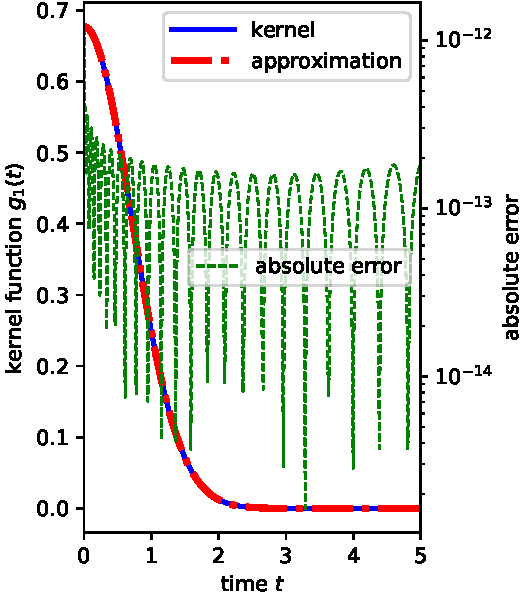
\includegraphics{PIC/g1}
\caption{absolute error}
\end{subfigure}
\begin{subfigure}[b]{0.49\textwidth}
\centering
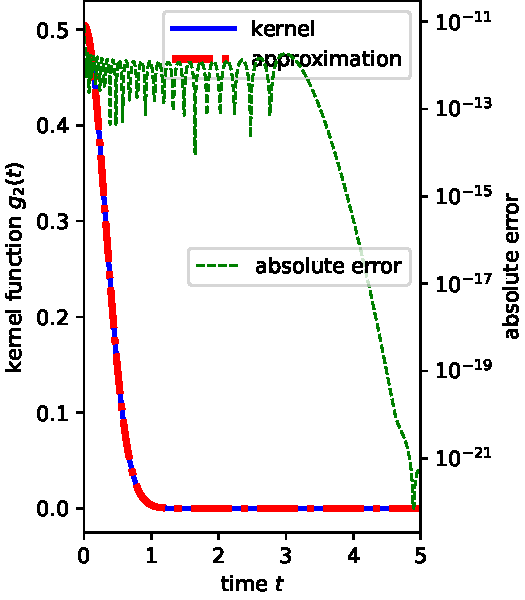
\includegraphics{PIC/g2}
\caption{absolute error}
\end{subfigure}
\end{figure}

Using the following parameters:
        nc = 4.
         n = 40.
     order = 800.
 precision = 684.
 tolerance = 1.0000e-12.
    kernel = 1.2*sqrt(1/pi)*exp(-t^2).

M = 
+3.1408564644840428e+01+2.4419195061753636e-204j
-1.6706983140997441e+01+1.6944936341891648e+01j
-1.6706983140997441e+01-1.6944936341891648e+01j
+4.3117593746835351e-03+1.0182620511730521e+01j
+4.3117593746835351e-03-1.0182620511730521e+01j
+1.5801217025257626e+00+1.7151347706207849e+00j
+1.5801217025257626e+00-1.7151347706207849e+00j
-2.5283515424182218e-01+3.6580452129545922e-02j
-2.5283515424182218e-01-3.6580452129545922e-02j
+9.6864499480377557e-03+4.3130572825140741e-03j
+9.6864499480377557e-03-4.3130572825140741e-03j
-7.0188900179621449e-05+5.9181046455302063e-05j
-7.0188900179621449e-05-5.9181046455302063e-05j
S = 
+4.5016919366209596e+00-0.0000000000000000e+00j
+4.4950837272609609e+00+1.0395441820843294e+00j
+4.4950837272609609e+00-1.0395441820843294e+00j
+4.4749101704334056e+00-2.0949342266104529e+00j
+4.4749101704334056e+00+2.0949342266104529e+00j
+4.4400143885590264e+00+3.1851640805978376e+00j
+4.4400143885590264e+00-3.1851640805978376e+00j
+4.3879941466299011e+00-4.3376514748574726e+00j
+4.3879941466299011e+00+4.3376514748574726e+00j
+4.3138681929799541e+00-5.6015344176775130e+00j
+4.3138681929799541e+00+5.6015344176775130e+00j
+4.2046027378649198e+00+7.1006004448588689e+00j
+4.2046027378649198e+00-7.1006004448588689e+00j


Using the following parameters:
        nc = 2.
         n = 60.
     order = 800.
 precision = 1044.
 tolerance = 1.0000e-12.
    kernel = .4*sqrt(5/pi)*exp(-5*t^2).

M = 
+6.0218717426942279e+00+1.4362419538632482e+01j
+6.0218717426942279e+00-1.4362419538632482e+01j
-7.8895688897164868e+00+3.2240559090826211e+00j
-7.8895688897164868e+00-3.2240559090826211e+00j
+2.2797015886898708e+00+8.8649822336472972e-01j
+2.2797015886898708e+00-8.8649822336472972e-01j
-1.5812385534468196e-01+2.9191184324438230e-01j
-1.5812385534468196e-01-2.9191184324438230e-01j
-1.6437582106072690e-03+1.6960418050851949e-02j
-1.6437582106072690e-03-1.6960418050851949e-02j
+7.6424085578944063e-05+1.6850302286864095e-04j
+7.6424085578944063e-05-1.6850302286864095e-04j
S = 
+9.6866343601855860e+00+1.2046328869474987e+00j
+9.6866343601855860e+00-1.2046328869474987e+00j
+9.6530072014802286e+00-3.6349046934229232e+00j
+9.6530072014802286e+00+3.6349046934229232e+00j
+9.5835268922218706e+00-6.1329206717667075e+00j
+9.5835268922218706e+00+6.1329206717667075e+00j
+9.4728351525770442e+00+8.7631646660075901e+00j
+9.4728351525770442e+00-8.7631646660075901e+00j
+9.3094050935928543e+00-1.1638552294146715e+01j
+9.3094050935928543e+00+1.1638552294146715e+01j
+9.0629660627080142e+00+1.5040663840954302e+01j
+9.0629660627080142e+00-1.5040663840954302e+01j


